\section{System assessments}\label{sec:system_assessments}
The evaluation method defined in Section~\ref{sec:evaluation_instrument} is applied to the eleven primary systems selected in Sections~\ref{sec:taxonomy} and~\ref{sec:methodology}.
Each system is assessed by analysing the code of a representative task suite (T1--T4) and recording condition outcomes (C1--C9).
The code samples are available in Appendix D~\cite{kavadias2026qplSurveySupplementary}.
Per-system evidence summaries are in Subsection~\ref{subsec:system_assessments:per_system}.
Comparative analysis is in Subsection~\ref{subsec:system_assessments:comparative}.

Tower is excluded from the formal assessment; Subsection~\ref{subsec:system_assessments:tower_aside} includes it as a labelled reference point.
Findings are reported here; interpretation of RQ1 and RQ2 is in Section~\ref{sec:discussion}.

\subsection{Per-system evidence summaries}\label{subsec:system_assessments:per_system}
The following section records evaluation outcomes for each of the eleven assessed systems.
Each system receives a brief introduction, a task-by-condition outcome matrix, an aggregated condition-profile summary and an evaluation analysis paragraph.

\subsubsection{OpenQASM 3.0}\label{subsubsec:system_assessments:per_system:openqasm}
OpenQASM~3.0 is a quantum assembly language and intermediate representation designed to express gate-level programs for communication with quantum hardware~\cite{cross2022openqasm3}.

\begin{center}
    \small
    \begin{tabular}{@{}lccccccccc@{}}
        \toprule
        \textbf{Task} & \textbf{C1} & \textbf{C2} & \textbf{C3} & \textbf{C4} & \textbf{C5} & \textbf{C6} & \textbf{C7} & \textbf{C8} & \textbf{C9} \\
        \midrule
        T1$^{\dag}$   & F           & F           & F           & F           & F           & F           & P           & C           & C           \\
        T2$^{\dag}$   & F           & F           & F           & F           & F           & F           & P           & C           & F           \\
        T3            & F           & F           & F           & F           & F           & F           & P           & C           & C           \\
        T4            & F           & F           & F           & -           & F           & -           & P           & F           & F           \\
        \bottomrule
    \end{tabular}
    \footnotesize$^{\dag}$ Constructed example.
\end{center}

\begin{center}
    \paragraph{Aggregated condition profile}
    \small
    \begin{tabular}{@{}ccccccccc@{}}
        \addlinespace
        \toprule
        C1 & C2 & C3 & C4 & C5 & C6 & C7 & C8 & C9 \\
        \midrule
        F  & F  & F  & F  & F  & F  & P  & F  & F  \\
        \bottomrule
    \end{tabular}
\end{center}

\paragraph{Evaluation analysis}
The recorded outcomes place OpenQASM~3.0 at the Assembly tier.
C2, C3, C6 and C9 all record F, placing the system below the Framework minimum bar defined in Subsection~\ref{subsec:evaluation_instrument:gating}.
Each task is a linear sequence of named gate applications on explicit, indexed \texttt{qubit} registers.
In T1--T3, each construction terminates in an explicit \texttt{measure} step to declared \texttt{bit} variables.
T4 reduces to the minimal exhibit \texttt{qubit[2] q; h q[0]; cx q[0], q[1];} and the language offers no value-level alternative.
As a result, C1, C2, C3 and C5 record sustained F\@.

C4 is aggregated from T1--T3 and C6 is aggregated worst-case across T1--T4 per Subsection~\ref{subsec:evaluation_instrument:conditions}.
T1--T3 each write the reverse step in the source, namely the second Hadamard layer in T1, the diffusion inversion \texttt{h; x; cz; x; h} in T2 and the correction \texttt{inv @ phase(c)} in T3.
Uncomputation is the programmer's responsibility rather than a language service.

Two conditions vary across the suite and aggregate worst-case to F\@.
C9 records C in T1 and T3, where user-defined gates and modifier expressions provide gate-level abstraction, and records F in T2 and T4, which inline their gate sequences.
C8 records C in T1--T3, where interference is readable from gate idiom and source comments, and records F in T4, where entanglement reduces to a literal \texttt{cx} application.
The language admits gate-level descriptions of interference and entanglement without providing constructs that name them.

C7 records P sustained across T1--T4.
The representative suite uses only standard gates and does not exercise OpenQASM v3 hardware-control surfaces such as timing or pulse-level calibration constructs.
This deviates from the Assembly row of Table~\ref{tab:evaluation_instrument:expected_profile}, which expects F\@.
The canonical examples satisfy the Assembly-tier criteria without engaging v3's hardware-control extensions.

\subsubsection{QIR}\label{subsubsec:system_assessments:per_system:qir}
QIR is an LLVM-based quantum intermediate representation designed as a language- and hardware-agnostic interchange format between quantum front-end compilers and target platforms~\cite{qir_alliance_qir_spec_repo}.

\begin{center}
    \small
    \begin{tabular}{@{}lccccccccc@{}}
        \toprule
        \textbf{Task} & \textbf{C1} & \textbf{C2} & \textbf{C3} & \textbf{C4} & \textbf{C5} & \textbf{C6} & \textbf{C7} & \textbf{C8} & \textbf{C9} \\
        \midrule
        T1$^{\dag}$   & F           & F           & F           & F           & F           & -           & P           & C           & F           \\
        T2$^{\dag}$   & F           & F           & F           & F           & F           & -           & P           & C           & F           \\
        T3$^{\dag}$   & F           & F           & F           & F           & F           & -           & P           & F           & F           \\
        T4            & F           & F           & F           & -           & F           & -           & P           & F           & F           \\
        \bottomrule
    \end{tabular}
    \footnotesize$^{\dag}$ Constructed example.
\end{center}
\begin{center}
    \paragraph{Aggregated condition profile}
    \small
    \begin{tabular}{@{}ccccccccc@{}}
        \addlinespace
        \toprule
        C1 & C2 & C3 & C4 & C5 & C6 & C7 & C8 & C9 \\
        \midrule
        F  & F  & F  & F  & F  & -  & P  & F  & F  \\
        \bottomrule
    \end{tabular}
\end{center}

\paragraph{Evaluation analysis}
The recorded outcomes place QIR at the IR tier.
C2, C3 and C9 record F across T1--T4 and C6 records no evidence in the representative suite.
The authoring surface is an LLVM-IR module: each task is an SSA function body in which quantum operations are expressed as named runtime intrinsic calls over opaque \texttt{\%Qubit*} and \texttt{\%Result*} handles.
T4 reduces to two allocations followed by \texttt{\_\_quantum\_\_qis\_\_h\_\_body} on one handle and \texttt{\_\_quantum\_\_qis\_\_cnot\_\_body} on the pair.
The surface offers no value-level quantum primitives, so C1, C2, C3 and C5 record sustained F\@.
C4 records F in T1--T3 where the task carries a reversal step (second Hadamard layer, diffusion inversion, inverse-QFT decomposition), written out as repeated intrinsic calls; uncomputation is hand-coded in source rather than supplied by the lowering pipeline.

Two conditions show within-suite variability.
C8 records C in T1 and T2, where Deutsch--Jozsa and Grover follow as gate recipes annotated with interference comments and F in T3 and T4, where phase decomposition and entangling intent require amplitude reasoning at the intrinsic level.
C9 records F sustained: LLVM IR exposes \texttt{define} and \texttt{call} as composition primitives, but the examples show only flat sequences of \texttt{\_\_quantum\_\_qis\_\_*} intrinsics.

Relative to the IR row of Table~\ref{tab:evaluation_instrument:expected_profile}, QIR records C6 as unassessable and C7 as passing in the representative suite, which reflects coverage of the canonical snippets rather than an absence of language capability.

\subsubsection{Q-MLIR}\label{subsubsec:system_assessments:per_system:qmlir}
Q-MLIR extends MLIR with a quantum dialect to enable progressive lowering from quantum assembly representations to LLVM IR and hardware targets~\cite{McCaskey2021MLIRDialectQASM}.

\begin{center}
    \small
    \begin{tabular}{@{}lccccccccc@{}}
        \toprule
        \textbf{Task}  & \textbf{C1} & \textbf{C2} & \textbf{C3} & \textbf{C4} & \textbf{C5} & \textbf{C6} & \textbf{C7} & \textbf{C8} & \textbf{C9} \\
        \midrule
        \midrule
        T1$^{\dagger}$ & F           & F           & F           & F           & F           & F           & P           & C           & C           \\
        T2             & F           & F           & F           & C           & F           & F           & P           & F           & C           \\
        T3$^{\dagger}$ & F           & F           & F           & F           & F           & F           & P           & F           & C           \\
        T4$^{\dagger}$ & F           & F           & F           & --          & F           & F           & P           & F           & C           \\
        \bottomrule
    \end{tabular}
    \footnotesize$^{\dag}$ Constructed example.
\end{center}



\begin{center}
    \paragraph{Aggregated condition profile}
    \small
    \begin{tabular}{ccccccccc}
        \addlinespace
        C1 & C2 & C3 & C4 & C5 & C6 & C7 & C8 & C9 \\
        \midrule
        F  & F  & F  & F  & F  & F  & P  & F  & C  \\
        \bottomrule
    \end{tabular}
\end{center}

\paragraph{Evaluation analysis}
The recorded outcomes place Q-MLIR at the IR tier.
C1, C2, C3 and C5 record F across T1--T4.
The authoring surface is a qcor-style C++ kernel lowering through MLIR quantum dialects: each task is a \texttt{\_\_qpu\_\_}-annotated function over an explicit \texttt{qreg} handle allocated with \texttt{qalloc(N)}, in which quantum operations are written as ordinary gate calls over indexed qubits.
T4 reduces to the minimal exhibit \texttt{H(q[0]); CX(q[0], q[1]);} inside a \texttt{\_\_qpu\_\_ void bell(qreg q)} kernel; the surface offers no value-level quantum primitives.

Three conditions warrant per-condition reasoning.
C4 records F in T1 and T3, where reversal is written out as ordinary gate calls, and C in T2, where the Grover diffusion uses a structured \texttt{compute \{ \ldots \} action \{ \ldots \}} block that keeps compute/uncompute user-visible but explicit.
C8 records C in T1 (gate recipe with implicit interference) and F in T2--T4, where Grover's controlled phase plus diffusion, QPE's \texttt{CRZ} decomposition and Bell preparation's entangling intent require amplitude or entanglement reasoning.
C9 records C across T1--T4: \texttt{\_\_qpu\_\_} kernel definitions and direct calls provide subroutine composition at the gate-kernel level rather than value-level functional composition.

Relative to the IR row of Table~\ref{tab:evaluation_instrument:expected_profile}, Q-MLIR records C7 as passing and C9 as constrained in the representative suite.
This reflects the use of an abstract gate namespace and reusable \texttt{\_\_qpu\_\_} kernels, but it does not lift the remaining Framework-minimum conditions above sustained failure.

\subsubsection{Qiskit}\label{subsubsec:system_assessments:per_system:qiskit}
Qiskit is a Python-based quantum programming framework providing an in-memory circuit model and transpilation infrastructure for execution on quantum simulators and hardware backends~\cite{aleksandrowicz2019qiskit}.

\begin{center}
    \small
    \begin{tabular}{@{}lccccccccc@{}}
        \toprule
        \textbf{Task} & \textbf{C1} & \textbf{C2} & \textbf{C3} & \textbf{C4} & \textbf{C5} & \textbf{C6} & \textbf{C7} & \textbf{C8} & \textbf{C9} \\
        \midrule
        T1            & F           & F           & F           & F           & F           & F           & P           & C           & C           \\
        T2            & F           & F           & F           & F           & F           & F           & P           & C           & C           \\
        T3            & F           & F           & F           & F           & F           & F           & P           & C           & C           \\
        T4            & F           & F           & F           & -           & F           & -           & P           & F           & F           \\
        \bottomrule
    \end{tabular}
\end{center}

\begin{center}
    \paragraph{Aggregated condition profile}
    \small
    \begin{tabular}{@{}ccccccccc@{}}
        \addlinespace
        \toprule
        C1 & C2 & C3 & C4 & C5 & C6 & C7 & C8 & C9 \\
        \midrule
        F  & F  & F  & F  & F  & F  & P  & F  & C  \\
        \bottomrule
    \end{tabular}
\end{center}

\paragraph{Evaluation analysis}
The recorded outcomes place Qiskit at the Framework tier.
Under the C2 lens, the artefact model is a host-embedded Python DSL in which each task constructs a \texttt{QuantumCircuit(\ldots)} object and mutates it through ordinary method calls, with explicit qubit and classical register identities throughout (\texttt{qr[0]}, \texttt{ClassicalRegister}, \texttt{measure\_all()}).
T4 shows the most compact program in the suite \texttt{QuantumCircuit(2); circuit.h(0); circuit.cx(0, 1)} and it still requires explicit circuit construction.
Superposition is introduced through an explicit Hadamard call rather than a value construct, and reversal and measurement are written as ordinary code at the circuit level.

The algorithmic tasks exercise Qiskit’s framework affordances through circuit-level composition, including \texttt{qc.compose(\ldots)}, library Grover operators and appending an inverse QFT via \texttt{QFT(3, inverse=True)}.
These affordances operate on explicitly constructed circuits and do not provide a value-level alternative to circuit authoring.

Relative to Table~\ref{tab:evaluation_instrument:expected_profile}, Qiskit records C5 as failed because quantum and classical data remain separated by an explicit register and measurement interface.
Representative workflows require manual placement and alignment of \texttt{measure(\ldots)} statements with qubit identities, which extracts outcomes but does not abstract the observation boundary.
The interface is therefore manual wiring rather than a language service, keeping C5 at F\@.

\subsubsection{PennyLane}\label{subsubsec:system_assessments:per_system:pennylane}
PennyLane is a Python-based quantum machine learning framework providing differentiable quantum computing through QNodes integrated with classical autodifferentiation libraries~\cite{bergholm2018pennylane}.

\begin{center}
    \small
    \begin{tabular}{@{}lccccccccc@{}}
        \toprule
        \textbf{Task} & \textbf{C1} & \textbf{C2} & \textbf{C3} & \textbf{C4} & \textbf{C5} & \textbf{C6} & \textbf{C7} & \textbf{C8} & \textbf{C9} \\
        \midrule
        T1            & F           & F           & F           & F           & F           & F           & P           & C           & C           \\
        T2            & F           & F           & F           & F           & F           & F           & P           & C           & C           \\
        T3            & F           & F           & F           & C           & F           & -           & P           & C           & C           \\
        T4            & F           & F           & F           & -           & F           & -           & P           & F           & F           \\
        \bottomrule
    \end{tabular}
\end{center}

\begin{center}
    \paragraph{Aggregated condition profile}
    \small
    \begin{tabular}{@{}ccccccccc@{}}
        \addlinespace
        \toprule
        C1 & C2 & C3 & C4 & C5 & C6 & C7 & C8 & C9 \\
        \midrule
        F  & F  & F  & F  & F  & F  & P  & F  & C  \\
        \bottomrule
    \end{tabular}
\end{center}

\paragraph{Evaluation analysis}
PennyLane most closely matches the \textit{Framework} tier when the aggregated profile is compared against the expected condition signatures in Table~\ref{tab:evaluation_instrument:expected_profile}.
Across the task suite, the artefact model is a host-embedded Python circuit DSL in which quantum behaviour is authored by applying named operations to explicitly identified wires inside a device-bound callable, for example \texttt{qml.device}, \texttt{@qml.qnode} and \texttt{qml} operation primitives.
This commits the programmer to an explicit circuit-as-program representation rather than offering a value-level semantics in which superposition is manipulated as an ordinary value.

The representative constructions are largely recipe-driven.
T1 and T2 follow a standard “prepare, apply oracle, interfere, read out” structure, while T3 delegates significant structure to a library routine via \texttt{qml.QuantumPhaseEstimation(\ldots)}.
This relaxes C4 to constrained on that task without changing the underlying circuit artefact model.

Relative to the \textit{Framework} profile in Table~\ref{tab:evaluation_instrument:expected_profile}, PennyLane deviates on C5 and C8.
C5 is recorded as failed because representative workflows still require explicit staging between quantum code and classical control, for example returning \texttt{qml.probs} and performing classical post-processing.
C8 is recorded as failed because the task suite includes explicit entanglement construction, making entanglement awareness a necessary correctness concept rather than an optional interpretive layer.

\subsubsection{Q\#}\label{subsubsec:system_assessments:per_system:qsharp}
Q\# is a domain-specific quantum programming language designed for expressing quantum algorithms as structured callables with strong classical--quantum integration~\cite{MicrosoftQSharpOverview}.

\begin{center}
    \small
    \begin{tabular}{@{}lccccccccc@{}}
        \toprule
        \textbf{Task} & \textbf{C1} & \textbf{C2} & \textbf{C3} & \textbf{C4} & \textbf{C5} & \textbf{C6} & \textbf{C7} & \textbf{C8} & \textbf{C9} \\
        \midrule
        T1            & F           & F           & F           & C           & F           & F           & P           & C           & C           \\
        T2            & F           & F           & F           & C           & F           & F           & P           & C           & C           \\
        T3$^{\dag}$   & F           & F           & F           & C           & F           & F           & P           & F           & C           \\
        T4            & F           & F           & F           & -           & F           & -           & P           & F           & F           \\
        \bottomrule
    \end{tabular}
    \footnotesize$^{\dag}$ Constructed example.
\end{center}

\begin{center}
    \paragraph{Aggregated condition profile}
    \small
    \begin{tabular}{@{}ccccccccc@{}}
        \addlinespace
        \toprule
        C1 & C2 & C3 & C4 & C5 & C6 & C7 & C8 & C9 \\
        \midrule
        F  & F  & F  & C  & F  & F  & P  & F  & C  \\
        \bottomrule
    \end{tabular}
\end{center}

\paragraph{Evaluation analysis}
Q\# most closely matches the \textit{Framework} tier when the aggregated condition profile is compared against the expected signatures in Table~\ref{tab:evaluation_instrument:expected_profile}.
Across the task suite, Q\# retains circuit- and qubit-explicit commitments in C1--C3 and an explicit observation boundary (C6=F).
Backend-specific concerns remain optional in the representative constructions (C7=P) and reusable algorithmic structure is available at the operation level (C9=C).

The representative artefact model is a standalone quantum language in which programs allocate qubits and apply typed operations.
Reversible structure is expressed through language constructs and functors, including \texttt{use} allocation, \texttt{within \{...\} apply \{...\}} and \texttt{Adjoint} and \texttt{Controlled} forms.
This supports structured reversal without requiring manual duplication of inverse gate sequences, yielding C4=C across the main algorithmic tasks.

Relative to the \textit{Framework} profile in Table~\ref{tab:evaluation_instrument:expected_profile}, Q\# falls at the constrained end of the permitted range for C5 and C8.
C5 is recorded as failed because representative workflows require an explicit boundary between quantum routines and classical control, with measurement results returned as classical values and consumed by classical loops and conditionals.
C8 is recorded as failed because the task suite includes phase-estimation structure and explicit entanglement construction, and representative implementations require phase-parameter reasoning for correctness rather than only invoking a provided black-box routine.

\subsubsection{Silq}\label{subsubsec:system_assessments:per_system:silq}
Silq is a standalone statically typed quantum programming language whose defining contribution is compiler-managed automatic uncomputation~\cite{bichsel2020silq}.

\begin{center}
    \small
    \begin{tabular}{@{}lccccccccc@{}}
        \toprule
        \textbf{Task} & \textbf{C1} & \textbf{C2} & \textbf{C3} & \textbf{C4} & \textbf{C5} & \textbf{C6} & \textbf{C7} & \textbf{C8} & \textbf{C9} \\
        \midrule
        T1            & F           & C           & C           & C           & C           & C           & P           & C           & P           \\
        T2            & F           & C           & C           & C           & C           & C           & P           & C           & P           \\
        T3$^{\dag}$   & F           & C           & C           & -           & C           & C           & P           & F           & P           \\
        T4$^{\dag}$   & F           & C           & C           & -           & C           & C           & P           & C           & P           \\
        \bottomrule
    \end{tabular}
    \footnotesize$^{\dag}$ Constructed example.
\end{center}

\begin{center}
    \paragraph{Aggregated condition profile}
    \small
    \begin{tabular}{@{}ccccccccc@{}}
        \addlinespace
        \toprule
        C1 & C2 & C3 & C4 & C5 & C6 & C7 & C8 & C9 \\
        \midrule
        F  & C  & C  & C  & C  & C  & P  & F  & P  \\
        \bottomrule
    \end{tabular}
\end{center}

\paragraph{Evaluation analysis}
Silq most closely matches the \textit{High-level} tier when the aggregated condition profile is compared against the expected signatures in Table~\ref{tab:evaluation_instrument:expected_profile}.
Silq supports ordinary program-level composition, keeps hardware adjacency optional and reduces several low-level obligations to constrained surface vocabulary rather than circuit plumbing.

The representative artefact model is a standalone language in which quantum data is manipulated directly as typed values, with control flow and abstraction expressed using ordinary functions.
Representative code uses program-level routines such as \texttt{groverDiffusion(cand)} and extracts classical outcomes through a builtin measurement operation such as \texttt{measure(cand)}.
This differs from framework-style circuit construction in that the primary surface is a program over quantum-typed data rather than an object that is assembled and then executed.

Across the task suite, the evidence shows reuse and encapsulation rather than inlined gate scripting.
T1 and T2 package algorithm structure as parameterised routines and use ordinary composition when invoking the oracle and diffusion components.
T4 is expressed as a reusable \texttt{bell\_pair} routine returning a pair that can be consumed by other code.
Measurement remains a required step for extracting classical outcomes, but it appears as a single builtin operation rather than explicit wiring of classical registers or measurement bookkeeping, which supports the constrained judgement on C6.

T3 drives the remaining tier constraint by requiring explicit phase reasoning and a concrete inverse-QFT decomposition, forcing a C8 failure even though the rest of the surface reads as program-like.
Relative to the \textit{High-level} expected profile in Table~\ref{tab:evaluation_instrument:expected_profile}, the primary deviations are C1 and C8.
C1 is recorded as failed because superposition is still introduced through explicit \texttt{H} applications on addressed components.
C8 is recorded as failed because representative phase estimation requires explicit phase-parameter reasoning rather than remaining purely recipe-level.

\subsubsection{Qmod (Classiq)}\label{subsubsec:system_assessments:per_system:qmod}
Qmod is a high-level quantum domain-specific language embedded in Python, designed to express algorithmic intent through quantum-native types and a synthesis engine that handles gate-level realisation~\cite{vax2025qmodexpressivehighlevelquantum}.

\begin{center}
    \small
    \begin{tabular}{@{}lccccccccc@{}}
        \toprule
        \textbf{Task} & \textbf{C1} & \textbf{C2} & \textbf{C3} & \textbf{C4} & \textbf{C5} & \textbf{C6} & \textbf{C7} & \textbf{C8} & \textbf{C9} \\
        \midrule
        T1            & C           & C           & C           & C           & C           & -           & P           & C           & P           \\
        T2            & C           & C           & C           & C           & C           & C           & P           & C           & P           \\
        T3$^{\dag}$   & F           & C           & C           & F           & C           & C           & P           & F           & P           \\
        T4            & F           & C           & C           & -           & C           & C           & P           & C           & P           \\
        \bottomrule
    \end{tabular}
    \footnotesize$^{\dag}$ Constructed example.
\end{center}

\begin{center}
    \paragraph{Aggregated condition profile}
    \small
    \begin{tabular}{@{}ccccccccc@{}}
        \addlinespace
        \toprule
        C1 & C2 & C3 & C4 & C5 & C6 & C7 & C8 & C9 \\
        \midrule
        F  & C  & C  & F  & C  & C  & P  & F  & P  \\
        \bottomrule
    \end{tabular}
\end{center}

\paragraph{Evaluation analysis}
Qmod most closely matches the \textit{High-level} tier when the aggregated condition profile is compared against the expected signatures in Table~\ref{tab:evaluation_instrument:expected_profile}.
Qmod supports ordinary subroutine composition, keeps hardware adjacency optional and presents representative code as functions over typed quantum objects rather than direct circuit-object mutation.

The representative artefact model is a typed, quantum-explicit programming surface with dedicated role annotations and callable types.
Representative examples use constructs such as \texttt{qfunc} and \texttt{qperm} explicit allocation via \texttt{allocate(res)}, and higher-order composition through \texttt{QCallable} parameters.
Across the task suite, higher-level structure is expressed through reusable components rather than inlined circuit construction.
T1 packages the Deutsch--Jozsa core as a conjugation pattern using \texttt{within\_apply} around \texttt{hadamard\_transform(x)} and \texttt{phase\_oracle(\ldots)}.
T2 expresses iteration through \texttt{power(r,\{...\})} and delegates the Grover iterate structure to a library combinator \texttt{grover\_operator(\ldots)}.
The observation boundary remains explicit where outcomes are extracted, including via output parameters and explicit \texttt{measure(count)} in the constructed phase-estimation listing.

T3 drives the remaining tier constraints by requiring gate-level decomposition and phase-parameter management, including an explicit inverse-QFT construction and controlled phase powers.
Relative to the \textit{High-level} expected profile in Table~\ref{tab:evaluation_instrument:expected_profile}, the primary deviations are C1, C4 and C8.
C1 is recorded as failed because superposition is still introduced through explicit Hadamard applications on addressed elements.
C4 is recorded as failed because the representative phase-estimation construction requires manual inverse-QFT decomposition as ordinary code.
C8 is recorded as failed because representative phase estimation and Bell-state preparation require explicit phase and entanglement understanding for correctness rather than remaining purely recipe-level.

\subsubsection{Quff}\label{subsubsec:system_assessments:per_system:quff}
Quff is a scripting-language-style quantum programming language with a hybrid quantum--classical execution model and runtime-managed automatic uncomputation on variable scope exit~\cite{wright2024quff}.

\begin{center}
    \small
    \begin{tabular}{@{}lccccccccc@{}}
        \toprule
        \textbf{Task} & \textbf{C1} & \textbf{C2} & \textbf{C3} & \textbf{C4} & \textbf{C5} & \textbf{C6} & \textbf{C7} & \textbf{C8} & \textbf{C9} \\
        \midrule
        T1$^{\dag}$   & F           & C           & F           & C           & C           & C           & P           & C           & P           \\
        T2            & F           & C           & F           & C           & C           & C           & P           & C           & P           \\
        T3$^{\dag}$   & F           & C           & F           & C           & C           & C           & P           & F           & P           \\
        T4$^{\dag}$   & F           & C           & F           & -           & C           & C           & P           & C           & P           \\
        \bottomrule
    \end{tabular}
    \footnotesize$^{\dag}$ Constructed example.
\end{center}

\begin{center}
    \paragraph{Aggregated condition profile}
    \small
    \begin{tabular}{@{}ccccccccc@{}}
        \addlinespace
        \toprule
        C1 & C2 & C3 & C4 & C5 & C6 & C7 & C8 & C9 \\
        \midrule
        F  & C  & F  & C  & C  & C  & P  & F  & P  \\
        \bottomrule
    \end{tabular}
\end{center}

\paragraph{Evaluation analysis}
Quff most closely matches the \textit{Framework} tier when the aggregated condition profile is compared against the expected signatures in Table~\ref{tab:evaluation_instrument:expected_profile}.
The representative artefact model is a scripting-language-like program surface that accumulates quantum operations through explicit quantum blocks and gate-level primitives, for example \texttt{H:(var q = 0u\{n\}) \{...\}}, indexed register access \texttt{q[i]} and explicit result extraction via \texttt{measure(q)}.
This supports a program-first workflow while retaining overt register identity and gate-idiom initiation of superposition, so the surface does not cross into the high-level profile.

Across the task suite, Quff consistently expresses algorithms as ordinary functions and control flow rather than circuit-object mutation, including higher-order use such as passing an oracle \texttt{f} into \texttt{grover(f, n)} and invoking it as \texttt{f(q)}.
Uncomputation support is present but remains a visible programming obligation, for example the explicit inversion step \texttt{invertF(f, q)} in Grover and \texttt{invertF(qft, count)} in phase estimation, prevents a fully implicit clean-up story.
Result extraction is explicit but compact, with a single builtin boundary such as \texttt{measure(query)} or \texttt{measure(count)}, which supports a higher level rather than more circuit-plumbing-heavy pattern.
The phase-estimation construction still forces explicit phase reasoning in the representative listing, for example the explicit \texttt{phase(pi/4, t[0])} unitary and the controlled-power iteration pattern, which drives C8 failure in the aggregate.

Relative to the \textit{Framework} expected profile in Table~\ref{tab:evaluation_instrument:expected_profile}, Quff’s main upward pressures are C2, C4 and C6, reflecting a programmatic surface with structured inversion and a compact measurement boundary.
However, the tier allocation remains limited by sustained quantum-explicit discriminators, particularly C1 and C3 and by the phase-estimation requirement that keeps C8 at F in representative constructions.

\subsubsection{Qutes}\label{subsubsec:system_assessments:per_system:qutes}
Qutes is a standalone imperative quantum programming language with a static compiler frontend and scope-bounded liveness-guided automatic uncomputation~\cite{faro2025qutes,reversiblelifetime2026}.


\begin{center}
    \small
    \begin{tabular}{@{}lccccccccc@{}}
        \toprule
        \textbf{Task} & \textbf{C1} & \textbf{C2} & \textbf{C3} & \textbf{C4} & \textbf{C5} & \textbf{C6} & \textbf{C7} & \textbf{C8} & \textbf{C9} \\
        \midrule
        T1            & F           & C           & F           & P           & C           & C           & P           & C           & P           \\
        T2            & P           & P           & P           & P           & P           & P           & P           & P           & P           \\
        T3$^{\dag}$   & F           & C           & F           & C           & C           & C           & P           & F           & P           \\
        T4$^{\dag}$   & F           & C           & F           & -           & C           & C           & P           & C           & P           \\
        \bottomrule
    \end{tabular}
    \footnotesize$^{\dag}$ Constructed example.
\end{center}

\begin{center}
    \paragraph{Aggregated condition profile}
    \small
    \begin{tabular}{@{}ccccccccc@{}}
        \addlinespace
        \toprule
        C1 & C2 & C3 & C4 & C5 & C6 & C7 & C8 & C9 \\
        \midrule
        F  & C  & F  & C  & C  & C  & P  & F  & P  \\
        \bottomrule
    \end{tabular}
\end{center}

\paragraph{Evaluation analysis}
Qutes most closely matches the \textit{Framework} tier when the aggregated condition profile is compared against the expected signatures in Table~\ref{tab:evaluation_instrument:expected_profile}.
The representative artefact model is a standalone language whose surface can range from explicitly quantum programs with typed qubit arrays and gate-level operations to classical-looking code that invokes quantum search implicitly.
This yields a mixed task profile in which one representative construction (Grover) is quantum-implicit in appearance, while the remaining tasks retain explicit quantum vocabulary and resource identity.

Across the task suite, T2 is the outlier: the Grover workload is expressed as a native membership test, for example, \texttt{"01" in b}, with no visible qubits, circuit artefacts, measurement API or amplitude reasoning, and all conditions record P in that task.
By contrast, T1 and T4 are written in explicitly quantum terms, including explicit quantum state initialisation (e.g. \texttt{$\ket{+}$} and \texttt{$\ket{-}$}), explicit quantum types (e.g. \texttt{qubit[]}) and explicit gate constructs such as \texttt{mcx}, \texttt{H} and \texttt{CX}.
Result extraction is present even when it is not framed as a low-level measurement API, for example via assignments like \texttt{bool result = q} and explicit \texttt{measure(q)}, which supports the constrained judgement on C6.

Relative to the \textit{Framework} expected profile in Table~\ref{tab:evaluation_instrument:expected_profile}, Qutes is pulled upward by the existence of a task that eliminates quantum marking, qubit identity and measurement boundary concerns at the surface (T2).
However, the tier allocation remains limited by sustained quantum-explicit discriminators in other representative tasks, particularly C1 and C3 and by the phase-estimation construction which keeps C8 at F\@.

\subsubsection{Qwerty}\label{subsubsec:system_assessments:per_system:qwerty}
Qwerty is a basis-oriented high-level quantum programming language and compiler toolchain designed to express algorithms through basis-structured primitives and compilation to hardware backends~\cite{adams2024qwerty}.

\begin{center}
    \small
    \begin{tabular}{@{}lccccccccc@{}}
        \toprule
        \textbf{Task} & \textbf{C1} & \textbf{C2} & \textbf{C3} & \textbf{C4} & \textbf{C5} & \textbf{C6} & \textbf{C7} & \textbf{C8} & \textbf{C9} \\
        \midrule
        T1            & C           & P           & P           & P           & F           & F           & P           & C           & P           \\
        T2            & C           & P           & P           & P           & F           & C           & P           & P           & P           \\
        T3            & C           & C           & C           & C           & F           & C           & P           & F           & P           \\
        T4            & C           & C           & C           & -           & F           & C           & P           & C           & P           \\
        \bottomrule
    \end{tabular}
\end{center}

\begin{center}
    \paragraph{Aggregated condition profile}
    \small
    \begin{tabular}{@{}ccccccccc@{}}
        \addlinespace
        \toprule
        C1 & C2 & C3 & C4 & C5 & C6 & C7 & C8 & C9 \\
        \midrule
        C  & C  & C  & C  & F  & F  & P  & F  & P  \\
        \bottomrule
    \end{tabular}
\end{center}

\paragraph{Evaluation analysis}
Qwerty most closely matches the \textit{Framework} tier when the aggregated condition profile is compared against the expected signatures in Table~\ref{tab:evaluation_instrument:expected_profile}.
Across the task suite, Qwerty provides a programmatic, basis-oriented surface in which algorithms are expressed as Python functions composed through basis translations and oracle lifting.
In T1 and T2, representative code composes classical predicates into phase oracles via \texttt{oracle.sign} and expresses interference and diffusion through basis-translation operators such as \texttt{pm**N >> std**N} and \texttt{'p'**N >> -'p'**N}.
These constructions avoid circuit-object manipulation and do not require manual uncompute steps in the representative snippets (C4=P in T1 and T2), but they still require explicit staging via \texttt{@qpu} and explicit measurement operators to get classical results, which keeps C5 and C6 at failure or constrained outcomes.
T4 further shows that entanglement can be introduced as an explicit superposition literal (\texttt{'00' + '11'}) and then consumed as a compositional unit via a separate routine.

T3 drives the remaining tier constraint by requiring an explicit phase-estimation structure, including a controlled-power pattern and an explicit inverse-QFT via \texttt{fourier[prec].measure} and by requiring phase or eigenvalue reasoning for correctness.
As a result, while Qwerty’s basis-oriented primitives reduce gate-level expression burden, the tier assignment remains bounded by mandatory quantum marking, explicit observation boundaries and the persistence of phase reasoning in representative workloads.

\subsection{Tower reference aside}\label{subsec:system_assessments:tower_aside}
\textit{The following is an informal aside.
Tower was excluded from primary assessment.
Its outcomes do not contribute to the comparative analysis or the conclusions in Section~\ref{sec:discussion}.
It is included as a labelled reference point for contrasting system approaches and evidence limitations.}
Tower is retained as a labelled contrast because it develops a programming model for pointer-based quantum data structures and dynamic memory allocation, treating correctness constraints under superposition as first-class language concerns~\cite{yuan2025foundationalabstractions}.
The formal development characterises three constraints shaping its data model, reversibility, history independence and bounded-time execution determined by classical parameters~\cite{yuan2025foundationalabstractions}.
Tower is excluded from the task-based assessment and does not contribute to the tier distribution or comparative analysis because it fails the maintenance-window criterion and does not provide task-aligned public documentation sufficient to implement T1--T4 in a comparable way~\cite{yuan2025foundationalabstractions}.
Figure~\ref{fig:pub_qpl_review:system_assessments:tower_list} provides a representative example of list manipulation in Tower~\cite{yuan2025foundationalabstractions}.

\begin{figure}[t]
    \centering
    \begin{lstlisting}[language={},basicstyle=\ttfamily\small,frame=single]
type list = ( uint , ptr<list>);

fun length_n {
    with {
        let is_empty <- xs == null;
    } do if is_empty {
        let out <- acc;
    } else with {
        let temp <- default<list>;
        *xs <-> temp;
        let next <- temp.2;
        let r <- acc + 1;
    } do {
        let out <- length_{n-1};
    }
    return out;
}
    \end{lstlisting}
    \caption{Tower list type and a bounded recursive function computing list length, illustrating pointer-based data structure manipulation under an explicit reversible update discipline\cite{yuan2025foundationalabstractions}.}
    \label{fig:pub_qpl_review:system_assessments:tower_list}
\end{figure}

\subsection{Result summary}\label{subsec:system_assessments:summary}
Table~\ref{tab:system_assessments:system_summary} presents tier assignment and condition outcomes (C1--C9) for all eleven primary systems.

\begin{table*}[htbp*]
    \centering
    \caption{System assessment results. Tier is assigned by justified profile match under the task/condition instrument. Outcomes are recorded as F (fail), C (constrained), P (pass) or `-' (unassessable).}
    \label{tab:system_assessments:system_summary}
    \small
    \begin{tabular}{@{}lcccccccccc@{}}
        \toprule
        \textbf{System} & \textbf{Tier} & \textbf{C1} & \textbf{C2} & \textbf{C3} & \textbf{C4} & \textbf{C5} & \textbf{C6} & \textbf{C7} & \textbf{C8} & \textbf{C9} \\
        \midrule
        OpenQASM~3.0    & Assembly      & F           & F           & F           & F           & F           & F           & P           & F           & F           \\
        QIR             & IR            & F           & F           & F           & F           & F           & -           & P           & F           & F           \\
        Q-MLIR          & IR            & F           & F           & F           & F           & F           & F           & P           & F           & C           \\
        Qiskit          & Framework     & F           & F           & F           & F           & F           & F           & P           & F           & C           \\
        PennyLane       & Framework     & F           & F           & F           & F           & F           & F           & P           & F           & C           \\
        Q\#             & Framework     & F           & F           & F           & C           & F           & F           & P           & F           & C           \\
        Silq            & High-level    & F           & C           & C           & C           & C           & C           & P           & F           & P           \\
        Qmod            & High-level    & F           & C           & C           & F           & C           & C           & P           & F           & P           \\
        Quff            & Framework     & F           & C           & F           & C           & C           & C           & P           & F           & P           \\
        Qutes           & Framework     & F           & C           & F           & C           & C           & C           & P           & F           & P           \\
        Qwerty          & Framework     & C           & C           & C           & C           & F           & F           & P           & F           & P           \\
        \bottomrule
    \end{tabular}
\end{table*}

\subsection{Comparative analysis}\label{subsec:system_assessments:comparative}
Tier groupings throughout this subsection refer to the tier assignments reported in Table~\ref{tab:system_assessments:system_summary}.

\subsubsection{Condition pattern analysis}\label{subsubsec:system_assessments:condition_patterns}
Condition outcomes are analysed comparatively by examining how the aggregated profiles (C1--C9) cluster within and across tiers, and by identifying outliers where a condition behaves differently from the typical signature for a given tier.
Table~\ref{tab:system_assessments:system_summary} provides the primary reference for these comparisons, while Figure~\ref{fig:system_assessments:condition_heatmap} visualises the same outcomes as a full systems~$\times$~conditions matrix.
The purpose of this subsection is to report these observed patterns as results.

Across the recorded outcomes, two global patterns dominate the comparative matrix.
First, C7 (\emph{hardware concerns optional}) records P throughout the review set.
In the representative constructions, hardware-adjacent constraints do not appear as mandatory obligations at the authoring surface, so C7 does not act as a discriminator between tiers in Table~\ref{tab:system_assessments:system_summary}.
Second, the conditions tied most directly to a circuit- and qubit-explicit interface remain strongly constrained across tasks.
C2 (\emph{non-circuit primary artefact}) records predominantly F or C and C3 (\emph{qubit identity not user-visible}) predominantly records F\@.
This indicates that most representative implementations retain overt circuit artefacts and overt qubit handles even when other aspects of the programming surface are more program-like.

The required-knowledge condition C8 (\emph{no mandatory amplitude or entanglement reasoning}) exhibits a task-dependent pattern rather than uniform behaviour across the suite.
Deutsch--Jozsa (T1) consistently records C8 as constrained, while phase estimation (T3) records C8 as failed for the majority of systems.
Bell-state preparation (T4) splits between constrained and failed outcomes.
This task dependence is consistent with the role of phase estimation and explicit entanglement construction as recurring points where representative implementations surface amplitude-, phase- or entanglement-level reasoning requirements.

Tier separation in the recorded outcomes is driven primarily by whether systems can lift the \emph{discriminator conditions}, namely C2 (\emph{non-circuit primary artefact}), C3 (\emph{qubit identity not user-visible}), C6 (\emph{no measurement boundary}) and C9 (\emph{first-class composition}), above sustained failure.
Assembly and IR systems record uniform failures on these conditions, while Framework and High-level systems typically improve them only to constrained outcomes rather than to full passes.
Within the upper tiers, the most consistent improvements occur in the conditions associated with program structuring and reuse.
Systems assigned to the High-level tier record constrained or passing outcomes on first-class composition (C9) and improved outcomes on uncomputation support (C4) and observation handling (C6), but these gains coexist with persistent constraints on the artefact and qubit-identity conditions in representative code.

The review set also contains a clear paradigm outlier.
Qwerty is the only basis-oriented system in the primary set, and it is the only system whose aggregated profile records C1 as constrained rather than failed.
This shift co-occurs with sustained failures on the staging and observation boundary conditions (C5 and C6), so the profile reflects a surface that reduces some gate-idiom burden through basis-level primitives while still requiring explicit quantum marking and explicit result extraction.
A second outlier is coverage-related rather than paradigmatic.
QIR records “unassessable” outcomes for C6 in the representative suite, so its observation-boundary status should be interpreted as a limitation of the available task-aligned evidence rather than as a positive outcome.

Taken together, these patterns indicate that tier progression in the review set is characterised less by uniform improvement across all conditions than by selective relief on a subset of constraints, with persistent failure modes remaining visible in representative code even for the highest-assigned systems.
The comparative structure of the results is therefore captured by identifying which conditions remain uniformly constrained across the suite, which conditions improve only for specific paradigms and which task families concentrate the strongest failures.

\subsubsection{Constraint drivers and required-knowledge pressure}\label{subsubsec:system_assessments:constraint_drivers}
This subsection reports which conditions most commonly limit upward tier movement in the recorded outcomes.
A condition is treated as a \emph{constraint driver} when it remains at sustained failure or does not improve beyond constrained outcomes, even when other conditions improve.
The analysis prioritises the discriminator hierarchy introduced in Subsection~\ref{subsec:evaluation_instrument:gating}, focusing on C2 (\emph{non-circuit primary artefact}), C3 (\emph{qubit identity not user-visible}), C6 (\emph{no measurement boundary}) and C9 (\emph{first-class composition}).
To avoid attributing worst-case aggregation effects to language-level obligations, the comparative description draws on both the aggregated profiles in Table~\ref{tab:system_assessments:system_summary} and a task-wise view of outcomes across T1--T4.
Required-knowledge pressure is reported primarily through C8 (\emph{no mandatory amplitude or entanglement reasoning}).

Across tiers, the most persistent discriminator constraint is C3 (\emph{qubit identity not user-visible}).
For every task in the suite, the majority of systems record C3 as failed, with only a small minority of constrained outcomes and only isolated pass outcomes.
This places a hard ceiling on progression toward the quantum-implicit gate set, because implementations continue to surface qubit handles, indexing or explicit allocation and lifetime management even when program structure and reuse improve.

C2 (\emph{non-circuit primary artefact}) exhibits a similar, but less absolute, constraint pattern.
Upward movement is often expressed as a shift toward program-like organisation while still retaining circuit-centred authoring.

By contrast, C9 (\emph{first-class composition}) is not uniformly limiting.
In T1--T3, many systems record C9 as constrained or passing, indicating that routine-level composition is often achievable within the reviewed paradigms even when artefact and qubit-identity constraints persist.
The Bell-pair task is less diagnostic for C9, and it frequently records failures due to minimal constructions that do not require composition to express the task.

C6 (\emph{no measurement boundary}) improves more often than C2 and C3, but it does not reach uniform passes.
Across tasks, several systems record constrained outcomes on C6, reflecting interfaces that compress observation into a single operation while still requiring result extraction.
However, observation boundaries remain common, and unassessable cases occur where evidence does not exercise measurement, so C6 cannot be treated as consistently satisfied even when composition improves.

Required-knowledge pressure is most clearly expressed through C8 (\emph{no mandatory amplitude or entanglement reasoning}), which varies by task rather than remaining uniform across the suite.
Deutsch--Jozsa (T1) consistently records C8 as constrained, indicating that implementations typically remain followable as gate or basis recipes while still requiring some interference-level understanding to justify correctness.
By contrast, phase estimation (T3) concentrates the strongest failures, with the majority of systems recording C8 as failed.
Bell-state preparation (T4) also contributes sustained pressure, splitting between constrained and failed outcomes depending on whether the construction treats entanglement as an explicit correctness concept rather than as a byproduct of applying a known pattern.
This task dependence is important for interpreting aggregated profiles.
Under the worst-case aggregation rule, a single task that forces explicit phase-, amplitude- or entanglement-level reasoning is enough to drive the aggregated C8 outcome to failure even when other tasks remain recipe-followable.
Constructions reduce required-knowledge pressure in some task families, but they do not prevent it across the full suite, and the strongest pressure points recur at phase estimation and explicit entanglement construction.

A distinctive constraint pattern in the review set is driven by the basis-oriented paradigm represented by Qwerty.
In the suite, Qwerty expresses algorithm structure through basis-translation primitives and oracle lifting.
It does so without relying on explicit gate lists or circuit-object assembly.
This co-occurs with improved outcomes on C1 (\emph{superposition as value}) and with task-local passes on C2 and C3 in the Deutsch--Jozsa and Grover examples.
However, these constructions retain explicit staging and explicit observation boundaries.
This keeps C5 (\emph{no mandatory marking}) at failure, and it prevents C6 (\emph{no measurement boundary}) from improving beyond constrained outcomes.
Phase estimation remains the binding case for required-knowledge pressure in the same paradigm.
The Qwerty phase-estimation construction still requires explicit phase or eigenvalue reasoning for correctness, and it records C8 as failed.

This pattern contrasts with the dominant organisation used by the remaining systems.
Circuit- and IR-centred paradigms tend to fail C2 and C3 persistently.
In these paradigms, the primary artefact remains a circuit, tape or intrinsic sequence, and qubit identity remains explicit.
Program-first but qubit-explicit paradigms improve composition and in some cases compress observation to a builtin.
They still expose qubit handles or explicit quantum marking in code.
As a result, the discriminator conditions improve only to constrained outcomes.
The comparative result is that paradigm shifts can change which constraints are relieved first.
No paradigm in the review set eliminates the full discriminator gate set in representative constructions.

\subsubsection{Tier distribution}\label{subsubsec:system_assessments:tier_distribution}
Figure~\ref{fig:system_assessments:tier_distribution} shows the distribution of the eleven primary systems across tier assignments.
The review set spans four of the five tiers, with one Assembly system, two IR systems, six Framework systems and two High-level systems.
The Framework tier contains the largest group.
No reviewed system is assigned to the quantum-implicit tier under the recorded outcomes in Table~\ref{tab:system_assessments:system_summary}.

\begin{figure}[htbp*]
    \centering
    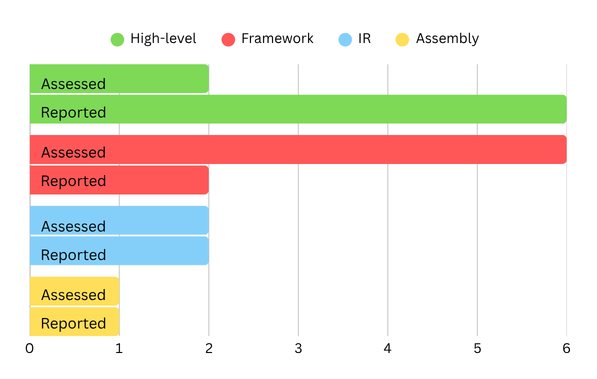
\includegraphics[width=0.8\linewidth]{../../figures/fig-system_assessments-tier_distribution}
    \caption{Distribution of primary systems across tier assignments.
    Also shows, for comparison, the systems’ taxonomy positioning as described in Section~\ref{sec:taxonomy}.}
    \label{fig:system_assessments:tier_distribution}
\end{figure}

\subsubsection{Systems $\times$ conditions heatmap}\label{subsubsec:system_assessments:condition_heatmap}
Figure~\ref{fig:system_assessments:condition_heatmap} presents the full outcome matrix as a heatmap, with systems ordered by tier and conditions C1--C9 in columns.
The heatmap provides a compact view of which conditions cluster by tier, and which conditions vary primarily by task family rather than by tier assignment.
Consistent with Table~\ref{tab:system_assessments:system_summary}, the strongest tier separation appears in the discriminator conditions C2, C3, C6 and C9, while C7 records uniformly permissive outcomes in the representative constructions.
The figure also makes outliers straightforward to identify, including the basis-oriented Qwerty profile and any unassessable cases that reflect evidence coverage limits rather than positive outcomes.

\begin{figure}[htbp*]
    \centering
    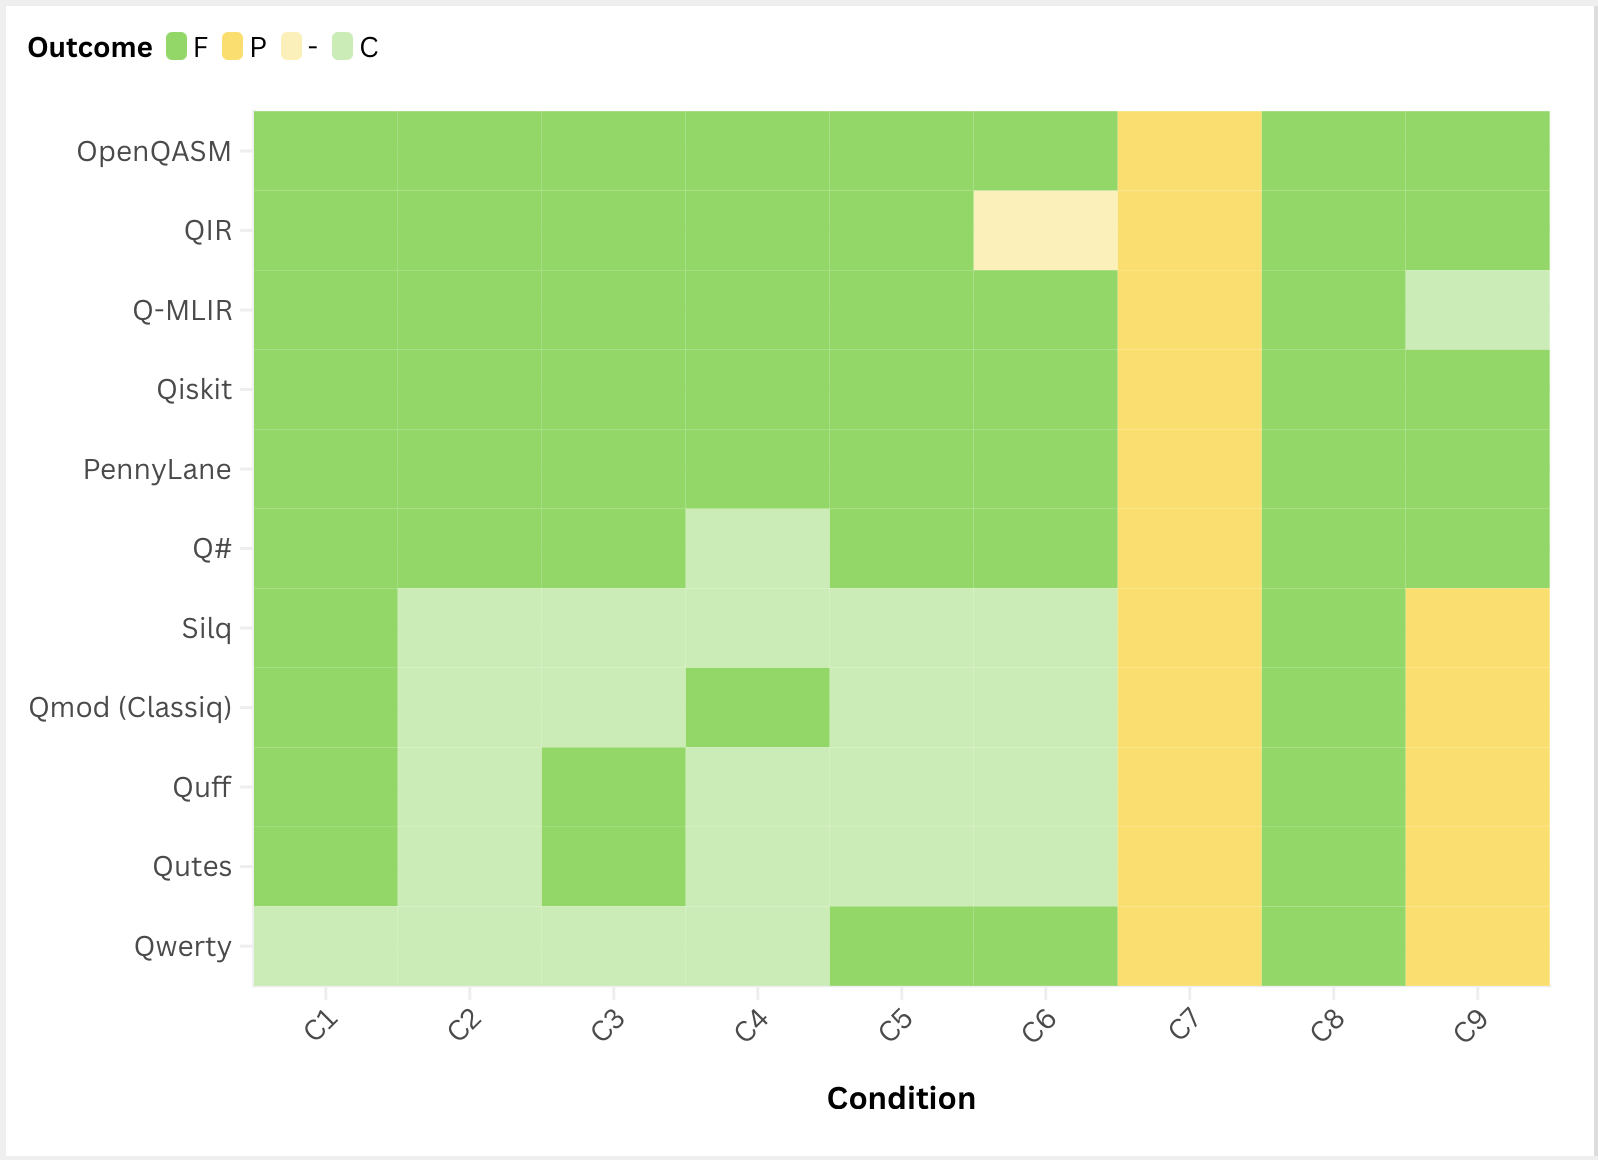
\includegraphics[width=0.95\linewidth]{../../figures/fig-system_assessments-condition_heatmap}
    \caption{Systems $\times$ conditions outcome heatmap (F/C/P/-).}
    \label{fig:system_assessments:condition_heatmap}
\end{figure}

\subsubsection{Quantum-implicit gap finding}\label{subsubsec:system_assessments:qi_gap}
No reviewed system satisfies the quantum-implicit gate set.
Representative constructions must achieve C2~=~P, C3~=~P, C6~=~P and C9~=~P for quantum-implicit classification.

The recorded outcomes show that at least one gate condition fails for every system in Table~\ref{tab:system_assessments:system_summary}.
Circuit- and IR-centred systems fail the artefact and identity conditions directly.
In representative OpenQASM, QIR, Q-MLIR, Qiskit and PennyLane constructions, the primary artefact remains an explicit gate sequence, an intrinsic sequence or a circuit object.
In the same constructions, qubit identity remains explicit through named registers, indexed wires or handle variables.
These systems also retain explicit observation boundaries.
Representative task constructions get classical results through explicit measurement operations or explicit probability readout interfaces.

Systems with more program-like organisation reduce some gate conditions only to constrained outcomes.
For Q\#, representative constructions improve the uncomputation condition through structured reversible blocks and explicit adjoint use.
The artefact, identity and observation boundary conditions remain failed in the representative suite.
For Silq and Qmod, representative code improves the artefact and identity conditions to constrained outcomes and improves composition to passing outcomes.
These systems still retain explicit marking and explicit observation boundaries.
They do not eliminate identity and artefact commitments across the full task suite.
For Quff and Qutes, representative code is organised as ordinary programs and composition records passing outcomes.
Qubit identity remains explicit through register values, indexing and quantum-marked regions.
Observation remains an explicit step even when compressed to a single builtin.

The basis-oriented paradigm represented by Qwerty changes which gate conditions improve first.
It does not satisfy the full gate set.
In the representative Deutsch--Jozsa and Grover constructions, Qwerty records task-local passes on C2 and C3 and records passing composition outcomes.
It retains explicit staging and explicit measurement operators.
This prevents C6 from reaching a pass outcome in the aggregated profile.
In phase estimation, the representative Qwerty construction still requires explicit phase or eigenvalue reasoning for correctness.
This co-occurs with an explicit observation boundary.

These failures are stated relative to the litmus test in Subsection~\ref{subsubsec:taxonomy:quantum_implicit}.
A language is quantum-implicit if a programmer with no prior instruction in quantum mechanics can learn it from its own documentation and examples.
They can implement and debug representative programs using ordinary mathematical and computational abstractions.
They can do so without needing to understand or use quantum-specific concepts such as qubits, gates, amplitudes or entanglement.
Under the recorded outcomes in Table~\ref{tab:system_assessments:system_summary}, the quantum-implicit tier is unoccupied.
The findings of this section are interpreted in Section~\ref{sec:discussion}.